  
\documentclass[10pt,a4paper,fleqn]{article} 
\usepackage[latin1]{inputenc} 
\usepackage[french]{babel} 
\usepackage{graphicx}
\graphicspath{{../figures/}}  
\usepackage[colorlinks=true,urlcolor=blue,citecolor=blue]{hyperref}  
\usepackage{amsmath} 
\usepackage{amssymb} 
\usepackage{rotating} 
% mcode options for matlab code insertion bw (for printing), numbered (line numbers), framed (frame around code blocks), useliterate (convert Matlab expressions to Latex ones), autolinebreaks (automatic code wraping, use it with caution 
\usepackage[literate]{mcode} 

\title{totoDemo version 0.1\\ default} 
\author{ lagrange } 
  
\begin{document} 
  
\maketitle 
  
tre

toto

%Please use this file to document your experiment 
%You can compile the report by setting the option 'report' to 1 (silent mode) or 2 (verbose mode) with generation of figures and table or -1 (silent mode) or -2 (verbose mode) for latex compilation only. 
  
This is the report to document the expCode project totoDemo using \LaTeX 
  
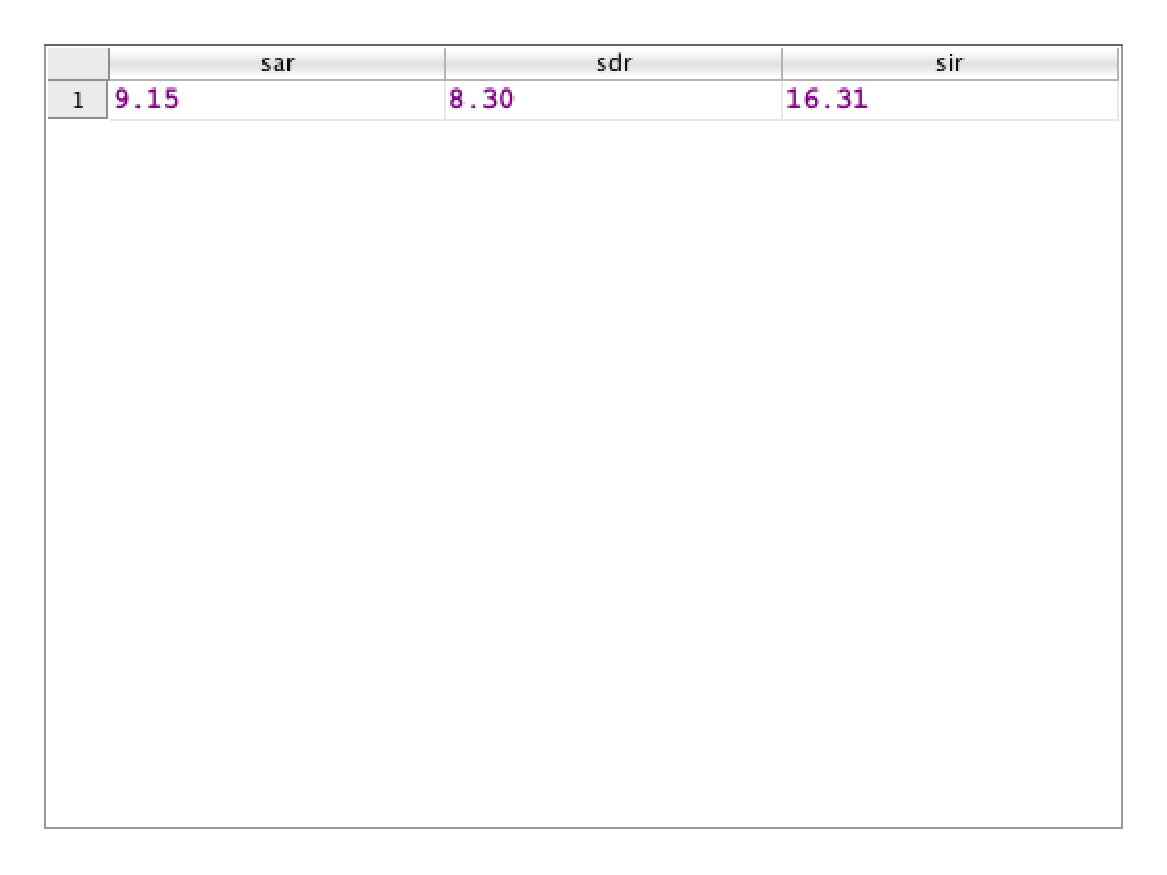
\includegraphics[width=\textwidth]{toto}


% expDisplayInsertionFlag DO NOT CLEAR (but move it where you want the code to be inserted)  
  
  
%\bibliographystyle{abbrvnat} 
%\bibliography{} 
  
\end{document} 
